\chapter{GDELT-Based Sentiment Analysis}
\label{chap:sentiment_news}

\begin{introduction}
This appendix describes the pipeline used to derive sector-specific sentiment labels from GDELT quotations. An ensemble of three large language models first annotates a representative subset of the data to produce a labelled dataset, and a lightweight FinBERT-based classifier is then trained on this dataset and applied to the full GDELT corpus to generate the sentiment features used in the main analysis.
\end{introduction}

Given the nature of this problem, understanding the causal impact of GDELT-derived quotes on sector performance, standard supervised learning approaches are not directly applicable, primarily due to the absence of a domain-specific labeled dataset. Moreover, although state-of-the-art sentiment classifiers such as FinBERT deliver strong general performance, they are not out-of-the-box designed to capture the nuanced, sector-specific signals that this task demands. A tailored modeling approach is therefore required.

To address this, a two-stage annotation and classification pipeline is proposed. In the first stage, a ensemble of large language models (LLMs) is employed to annotate a representative subset of the GDELT data, producing a high-quality labeled dataset that encodes the complex relationships between news events and sector-level market movements. In the second stage, a dedicated classifier is trained on this curated dataset and subsequently applied to the full GDELT corpus, enabling scalable and consistent sentiment labeling across the entire data universe.

\section{LLM-Based Annotation}
\label{sec:llm_annotation}

Because the GDELT news data are attributed to sectors via the dictionary-based filtering described in Section~\ref{subsec:gdelt_data}, a single quotation may be associated with one or more GICS sectors. Sentiment classification is therefore performed at the level of the quotation--sector pair: each unique combination receives an independent sentiment label (\textit{positive}, \textit{neutral}, or \textit{negative}) reflecting how the content of the quotation bears on that particular sector. For instance, a quotation linked to both the Energy and Real Estate sectors yields two separate classifications, one per sector. This design allows the same news event to carry different sentiment signals across sectors, which is more informative for downstream portfolio analysis.

Three LLMs, \texttt{meta-llama/Llama-3.1-8B-Instruct}, \texttt{google/gemma-7b-it}, and \texttt{Qwen/Qwen2.5-7B-Instruct}, were used as annotators, each receiving the same structured prompt. The final label for each article is determined by majority vote: if at least two of the three models agree, that label is assigned. This ensemble approach reduces the impact of individual model idiosyncrasies and provides a natural measure of annotation confidence through the degree of inter-model agreement. The annotation of the filtered GDELT subset yielded $\num{46729}$ labelled quotes, requiring approximately $\num{420}$ GPU-hours on a dual NVIDIA T4 setup.

\subsection{Prompt Design}
\label{sec:prompt}

The prompt, shown in Fig.~\ref{fig:GDELT_prompt}, was designed to standardize the classification task across models. It provides explicit classification rules, a definition of \textit{meaningful impact} (to minimize spurious positive or negative labels), and a structured JSON output format including a rationale and a confidence score. The sector label (\texttt{<SECTOR>}) and the news quotation (\texttt{<QUOTE>}) are injected at inference time, allowing the same prompt template to be reused across all quotations and sectors.

% moved fig fig:GDELT_prompt to the next section

\subsection{Vote Distribution}
\label{sec:vote_distribution}

Table~\ref{tab:GDELT_sentiment_votes_sector} reports the distribution of sentiment labels across sectors, broken down by the number of LLMs that agreed on the assigned label (1, 2, or 3 votes). High-vote counts indicate strong inter-model consensus and are generally associated with clearer, less ambiguous news content. The dominance of \textit{neutral} labels across all sectors are consistent with expectations, as the majority of news quotations either do not contain a direct causal link to sector performance or are too brief and decontextualized to allow a confident directional judgement.

% belongs to the previous section, but moved here
\begin{figure}[H]
\centering
\begin{tcolorbox}
\ttfamily\small
You are a financial-domain impact classifier for equity sectors. 

Your task is to analyze a GDELT news quote and classify the expected impact of the described events on a specific GICS sector.

$\ $

Classification Rules:

- "positive": the event is expected to benefit the sector (e.g., increased demand, revenue growth, cost reduction, regulatory advantage, market share gain).

- "negative": the event is expected to harm the sector (e.g., decreased demand, revenue loss, higher costs, regulatory pressure, operational disruption).

- "neutral": the event has no meaningful impact, is unrelated, or the impact is ambiguous/uncertain.

$\ $

Definition of "meaningful impact":

- There must be an explicit or implied causal link between the event and sector performance.

- The event should clearly suggest an effect on revenue, costs, operations, regulatory conditions, or valuation.

- Interpretation is allowed, but it must be logically justified with cause-effect reasoning.

$\ $

Non-meaningful impact:

- Mere mentions of companies, sectors, or locations without linkage to sector performance.

- Facts, statistics, or descriptions without explanation of consequences.

- Speculative statements with no plausible sector-level effect.

\begin{verbatim}
Output requirements:
Return a single JSON object exactly in the following format:
{
  "sector": <sector name>,
  "sentiment": <positive | negative | neutral>,
  "rationale": <3-5 sentence explanation linking the event to sector impact>,
  "confidence": <float between 0 and 1>
}
\end{verbatim}

- "rationale": 3-5 sentence explanation of why the impact label was chosen, highlighting the causal link.

- "confidence": float between 0.0 (very unsure) to 1.0 (very confident) representing your certainty.

- Default label is "neutral" if impact is unclear or not meaningful.

$\ $

Content to classify:

$\ $

Sector: \texttt{<SECTOR>}

Quote: \texttt{<QUOTE>}

$\ $

--- END OF CONTENT ---

$\ $

Classify strictly according to these rules. Output only the JSON object, nothing else.
\end{tcolorbox}
\caption{Prompt template used for sector-specific sentiment classification of GDELT quotes.}
\label{fig:GDELT_prompt}
\end{figure}



\begin{table}[ht]
\centering
\caption{Distribution of LLM sentiment votes (v) per sector for GDELT sector-specific sentiment classification, showing counts of quotes classified as positive, neutral, or negative based on agreement among three LLMs.}
\label{tab:GDELT_sentiment_votes_sector}
\renewcommand{\arraystretch}{1.2}
\begin{tabular}{|l|ccc|ccc|ccc|}
\hline
\multirow{2}{*}{\textbf{Sector}} 
& \multicolumn{3}{c|}{\textbf{Positive}} 
& \multicolumn{3}{c|}{\textbf{Neutral}} 
& \multicolumn{3}{c|}{\textbf{Negative}} \\

& \textbf{3v} & \textbf{2v} & \textbf{1v}
& \textbf{3v} & \textbf{2v} & \textbf{1v}
& \textbf{3v} & \textbf{2v} & \textbf{1v} \\
\hline

Energy & 118 & 108 & 601 & 2146 & 722 & 219 & 125 & 164 & 271 \\
Materials & 115 & 120 & 651 & 865 & 697 & 221 & 82 & 97 & 153 \\
Industrials & 190 & 240 & 694 & 1334 & 1004 & 397 & 218 & 187 & 308 \\
Consumer Discretionary & 143 & 141 & 638 & 1275 & 861 & 254 & 111 & 122 & 224 \\
Consumer Staples & 127 & 178 & 1338 & 1468 & 1641 & 309 & 86 & 126 & 228 \\
Health Care & 185 & 176 & 971 & 5865 & 1608 & 399 & 192 & 246 & 594 \\
Financials & 121 & 162 & 700 & 1708 & 923 & 397 & 262 & 263 & 379 \\
Information Technology & 211 & 246 & 1574 & 4882 & 2614 & 481 & 165 & 222 & 618 \\
Communication Services & 91 & 98 & 441 & 1770 & 883 & 209 & 87 & 109 & 196 \\
Utilities & 74 & 84 & 1103 & 1793 & 1324 & 244 & 143 & 178 & 319 \\
Real Estate & 116 & 146 & 1768 & 2002 & 2041 & 332 & 170 & 178 & 356 \\

\hline
\end{tabular}
\end{table}


\section{Ground-Truth Validation and Test Set Construction}
\label{sec:test_set}

Given the cost and scale of the annotation, a held-out test set was constructed through stratified sampling and independent validation by a stronger external model. Specifically, 20 quotes were sampled per sector, per sentiment category, and per agreement level (2 or 3 LLM votes), yielding a candidate pool of $20 \times 11 \times 3 \times 2 = \num{1320}$ quotes.

Each quote in this pool was independently classified by GPT-5.2 Chat (OpenAI)\footnote{\texttt{gpt-5.2-chat-latest}. As the model is a floating alias, results reflect the model capabilities at time of annotation (January 2026). \url{https://developers.openai.com/api/docs/models/gpt-5.2-chat-latest}.}, a larger and substantially more capable model than the three annotators, used here as an external referee rather than an annotator. Only articles where GPT-5.2 Chat's label agreed with the LLM majority vote were retained in the final test set, on the assumption that cross-system consensus is a reliable proxy for annotation quality. This filtering step produced a test set of $\num{969}$ articles.

It is worth noting that disagreement between GPT-5.2 Chat and the LLM ensemble does not necessarily imply that the ensemble label is incorrect. Manual inspection of a sample of disagreements revealed cases where the ensemble label was in fact more appropriate, for example, in the Health Care sector, GPT-5.2 Chat classified the quotation ``we will take care of them'' as \textit{positive}, whereas the three LLMs unanimously labelled it \textit{neutral}, which appears correct given the absence of any link to sector performance. This underscores the inherent difficulty of the task and the value of multi-model consensus for quality control.

Table~\ref{tab:GDELT_llm_agreement_sector} reports the rate at which GPT-5.2 Chat agreed with the LLM majority vote, broken down by sector, sentiment, and agreement level. The overall agreement rate was $63.9\%$ for articles with 2 LLM votes and $82.9\%$ for articles with 3 LLM votes, confirming that higher inter-LLM agreement is a strong signal of label reliability.

\begin{table}[ht]
\centering
\caption{Agreement between GPT-5.2 Chat and the LLM majority vote for GDELT sector-specific sentiment classification.}
\label{tab:GDELT_llm_agreement_sector}
\renewcommand{\arraystretch}{1.2}
\begin{tabular}{|l|l|c|c|}
\hline
\textbf{Sector} & \textbf{Sentiment} & \textbf{2 LLM votes} & \textbf{3 LLM votes} \\
\hline

\multirow{3}{*}{Energy}
& Negative & 12/20 (60\%) & 18/20 (90\%) \\
& Neutral  & 16/20 (80\%) & 20/20 (100\%) \\
& Positive & 8/20 (40\%) & 12/20 (60\%) \\
\hline

\multirow{3}{*}{Materials}
& Negative & 5/20 (25\%) & 14/20 (70\%) \\
& Neutral  & 14/20 (70\%) & 16/20 (80\%) \\
& Positive & 11/20 (55\%) & 14/20 (70\%) \\
\hline

\multirow{3}{*}{Industrials}
& Negative & 16/20 (80\%) & 14/20 (70\%) \\
& Neutral  & 17/20 (85\%) & 17/20 (85\%) \\
& Positive & 11/20 (55\%) & 15/20 (75\%) \\
\hline

\multirow{3}{*}{Consumer Discretionary}
& Negative & 16/20 (80\%) & 17/20 (85\%) \\
& Neutral  & 16/20 (80\%) & 17/20 (85\%) \\
& Positive & 12/20 (60\%) & 14/20 (70\%) \\
\hline

\multirow{3}{*}{Consumer Staples}
& Negative & 15/20 (75\%) & 17/20 (85\%) \\
& Neutral  & 17/20 (85\%) & 19/20 (95\%) \\
& Positive & 15/20 (75\%) & 19/20 (95\%) \\
\hline

\multirow{3}{*}{Health Care}
& Negative & 15/20 (75\%) & 17/20 (85\%) \\
& Neutral  & 9/20 (45\%) & 15/20 (75\%) \\
& Positive & 12/20 (60\%) & 18/20 (90\%) \\
\hline

\multirow{3}{*}{Financials}
& Negative & 13/20 (65\%) & 16/20 (80\%) \\
& Neutral  & 16/20 (80\%) & 20/20 (100\%) \\
& Positive & 10/20 (50\%) & 15/20 (75\%) \\
\hline

\multirow{3}{*}{Information Technology}
& Negative & 12/20 (60\%) & 13/20 (65\%) \\
& Neutral  & 10/20 (50\%) & 15/20 (75\%) \\
& Positive & 14/20 (70\%) & 20/20 (100\%) \\
\hline

\multirow{3}{*}{Communication Services}
& Negative & 5/20 (25\%) & 16/20 (80\%) \\
& Neutral  & 16/20 (80\%) & 19/20 (95\%) \\
& Positive & 6/20 (30\%) & 13/20 (65\%) \\
\hline

\multirow{3}{*}{Utilities}
& Negative & 15/20 (75\%) & 18/20 (90\%) \\
& Neutral  & 15/20 (75\%) & 18/20 (90\%) \\
& Positive & 9/20 (45\%) & 16/20 (80\%) \\
\hline

\multirow{3}{*}{Real Estate}
& Negative & 14/20 (70\%) & 19/20 (95\%) \\
& Neutral  & 14/20 (70\%) & 19/20 (95\%) \\
& Positive & 16/20 (80\%) & 17/20 (85\%) \\

\hline
\end{tabular}
\end{table}


\section{FinBERT-Based Sentiment Classifier}
\label{sec:finbert}

Applying the LLM ensemble to the full GDELT corpus ($\num{8602613}$ entries after filtering) would require approximately $\num{77500}$ GPU-hours, which is clearly infeasible. A lightweight supervised classifier is therefore trained on the labelled quotes and used to annotate the full dataset. Following the established practice in financial NLP (see Section~\ref{section:sentiment_analysis}), the model is built on \texttt{ProsusAI/FinBERT}, a BERT-base architecture pre-trained on financial corpora, which consistently achieves strong performance on financial sentiment benchmarks.

\subsection{Model Architecture}
\label{sec:architecture}

Because the labels are sector-specific, the model must condition its predictions on the sector associated with each article. Three variants are evaluated, all sharing the same FinBERT backbone and classifier head but differing in how sector information is encoded and injected:

\paragraph{Sector Embedding} The sector label is mapped to an integer ID and passed through a small learnable lookup table (\texttt{nn.Embedding}), producing a compact dense vector. This is the lightest-weight variant: the embedding is learned end-to-end from gradient signal, with no prior knowledge of sector semantics.

\paragraph{TF-IDF Embedding} Each sector is represented by its official GICS textual description\footnote{\url{https://www.msci.com/documents/1296102/29559863/GICS_structure_and_definitions_effective_close_of_March_17_2023.xlsx}}, vectorized using a TF-IDF encoder. This variant is inspired by the approach of Rizinski \emph{et~al.}~\cite{558b2} and sits between the other two in complexity, capturing sector-distinctive vocabulary without requiring a second neural encoder.

\paragraph{BERT Embedding} Each sector is represented by its official GICS textual description, encoded using a second, fully frozen FinBERT encoder. The mean-pooled hidden states provide a rich 768-dimensional semantic representation of each sector's domain. This is the most semantically expressive variant: sector similarity is captured implicitly through the pre-trained representations, without requiring the model to learn it from scratch.

$\ $

\noindent All three variants share the following architecture setup. News quotations are tokenized using FinBERT's vocabulary (max length 128 tokens). The \texttt{[CLS]} token's 768-dimensional hidden state serves as the primary text representation and is concatenated with the projected sector vector before the final linear classifier. Lower transformer layers remain frozen to preserve general linguistic representations, with the unfreezing threshold being treated as a hyperparameter. Optimization uses AdamW with differential learning rates, a smaller rate for the BERT encoder and a larger rate for the projection modules and classifier head. The loss function is Cross Entropy with label smoothing ($\epsilon = 0.1$).

\subsection{Training and Hyperparameter Tuning}
\label{sec:hyperparams}

Prior to training, the training data is undersampled by randomly drawing an equal number of articles per (sector, sentiment) combination, ensuring that the model is not biased towards more frequent sectors or sentiment classes. 

Model selection is performed using macro-F1 under 5-fold cross-validation on the training set, with the 969-article test set held out entirely. Each variant is subject to 25 trials of Bayesian hyperparameter search over the space defined in Table~\ref{tab:gdelt_hyperparams}. It covers three groups of hyperparameters. optimization dynamics are controlled by the encoder and head learning rates (\texttt{bert\_lr}, \texttt{head\_lr}), weight decay, and batch size. regularization is addressed through dropout and the number of unfrozen FinBERT layers (\texttt{unfrozen\_gte}), which also governs how much of the pre-trained backbone is adapted to the task. Finally, the dimensionality of the projected sector representation (\texttt{feature\_dim}) determines the size of the vector concatenated with the \texttt{[CLS]} token. For the TF-IDF variant, the vocabulary size (\texttt{tfidf\_dim}) is tuned as an additional parameter.

\begin{table}[ht]
  \centering
  \caption{Hyperparameter search space used for all three model variants in GDELT sector-specific sentiment classification (25 trials each).}
  \label{tab:gdelt_hyperparams}
  \renewcommand{\arraystretch}{1.2}
  \begin{tabular}{|l|l|l|l|}
    \hline
    \textbf{Hyperparameter} & \textbf{Type} & \textbf{Range / Values} & \textbf{Step} \\
    \hline
    \texttt{epochs}          & Integer           & $1$--$8$                                      & $1$           \\
    \texttt{bert\_lr}        & Log-uniform float & $10^{-6}$--$10^{-3}$                          & $\log$        \\
    \texttt{head\_lr}        & Log-uniform float & $10^{-6}$--$10^{-3}$                          & $\log$        \\
    \texttt{weight\_decay}   & Float             & $0.0$--$0.05$                                 & --            \\
    \texttt{bs}              & Categorical       & $\{8,\,16,\,32\}$                             & --            \\
    \texttt{dropout}         & Float             & $0.1$--$0.7$                                  & $0.05$        \\
    \texttt{unfrozen\_gte}   & Integer           & $4$--$11$                                     & $1$           \\
    \texttt{feature\_dim}    & Categorical       & $\{8,\,16,\,32,\,64,\,128\}$                  & --            \\
    \texttt{tfidf\_dim}      & Integer           & $100$--$1000$, $2000$--$15000$                & $100$, $1000$ \\
    \hline
\end{tabular}
\caption*{\footnotesize
Note: The \texttt{tfidf\_dim} hyperparameter is only applicable to the TF-IDF Embedding variant.
}
\end{table}

\subsection{Results}
\label{sec:gdeltresults}

The Sector Embedding variant achieved the best macro-F1 scores in cross-validation and on the test set, while also being the lightest of the three in terms of parameterization. The TF-IDF Embedding variant performed comparably but fell slightly short, and the BERT Embedding variant exhibited clear signs of overfitting, likely due to the relatively small training set and the additional parameters introduced by the frozen sector encoder. Based on predictive performance and inference efficiency, the Sector Embedding variant was selected as the final model for scoring the full GDELT corpus, with its results reported in this section.

The selected model was retrained on the full training set using the best hyperparameters found during tuning: 6 epochs, encoder learning rate of $10^{-5}$, head learning rate of $5 \times 10^{-5}$, weight decay of $0.005$, batch size of 16, dropout rate of $0.5$, the first 10 transformer layers frozen, and a feature dimension of 32.

Table~\ref{tab:GDELT_classification_report} and Fig.~\ref{fig:GDELT_confusion_matrix} report the classification report and confusion matrices for the training and held-out test sets, respectively. The model achieves a macro-F1 score of $0.83$ on the training set and $0.82$ on the test set, with no meaningful gap between the two, indicating good generalization without overfitting, which is further confirmed by the similar error patterns in the confusion matrices. These results are competitive with FinBERT-based models reported in the literature for financial sentiment classification tasks~\cite{rjhc3}. Among the three sentiment classes, \textit{neutral} is the most difficult to classify, as expected given its heterogeneous definition: it encompasses articles that are unrelated to the sector, ambiguous, or insufficiently causal. Positive and negative categories achieve broadly similar performance.

\begin{table}[H]
\centering
\caption{Classification report for the Sector Embedding variant in GDELT sector-specific sentiment classification, evaluated on the training set and the held-out test set.}
\label{tab:GDELT_classification_report}
\renewcommand{\arraystretch}{1.2}
\begin{tabular}{|l|lcccc|}
\hline
\textbf{Split} & \textbf{Class} & \textbf{Precision} & \textbf{Recall} & \textbf{F1-Score} & \textbf{Support} \\
\hline\hline
\multirow{6}{*}{Train}
& Negative     & 0.84 & 0.88 & 0.86 & 1463 \\
& Neutral      & 0.83 & 0.76 & 0.79 & 1463 \\
& Positive     & 0.83 & 0.85 & 0.84 & 1463 \\
\cline{2-6}
& Accuracy     &      &      & 0.83 & 4389 \\
& Macro avg    & 0.83 & 0.83 & 0.83 & 4389 \\
& Weighted avg & 0.83 & 0.83 & 0.83 & 4389 \\
\hline\hline
\multirow{6}{*}{Test}
& Negative     & 0.85 & 0.87 & 0.86 & 317 \\
& Neutral      & 0.81 & 0.74 & 0.77 & 355 \\
& Positive     & 0.78 & 0.85 & 0.81 & 297 \\
\cline{2-6}
& Accuracy     &      &      & 0.82 & 969 \\
& Macro avg    & 0.82 & 0.82 & 0.82 & 969 \\
& Weighted avg & 0.82 & 0.82 & 0.81 & 969 \\
\hline
\end{tabular}
\end{table}

\begin{figure}[H]
    \centering
    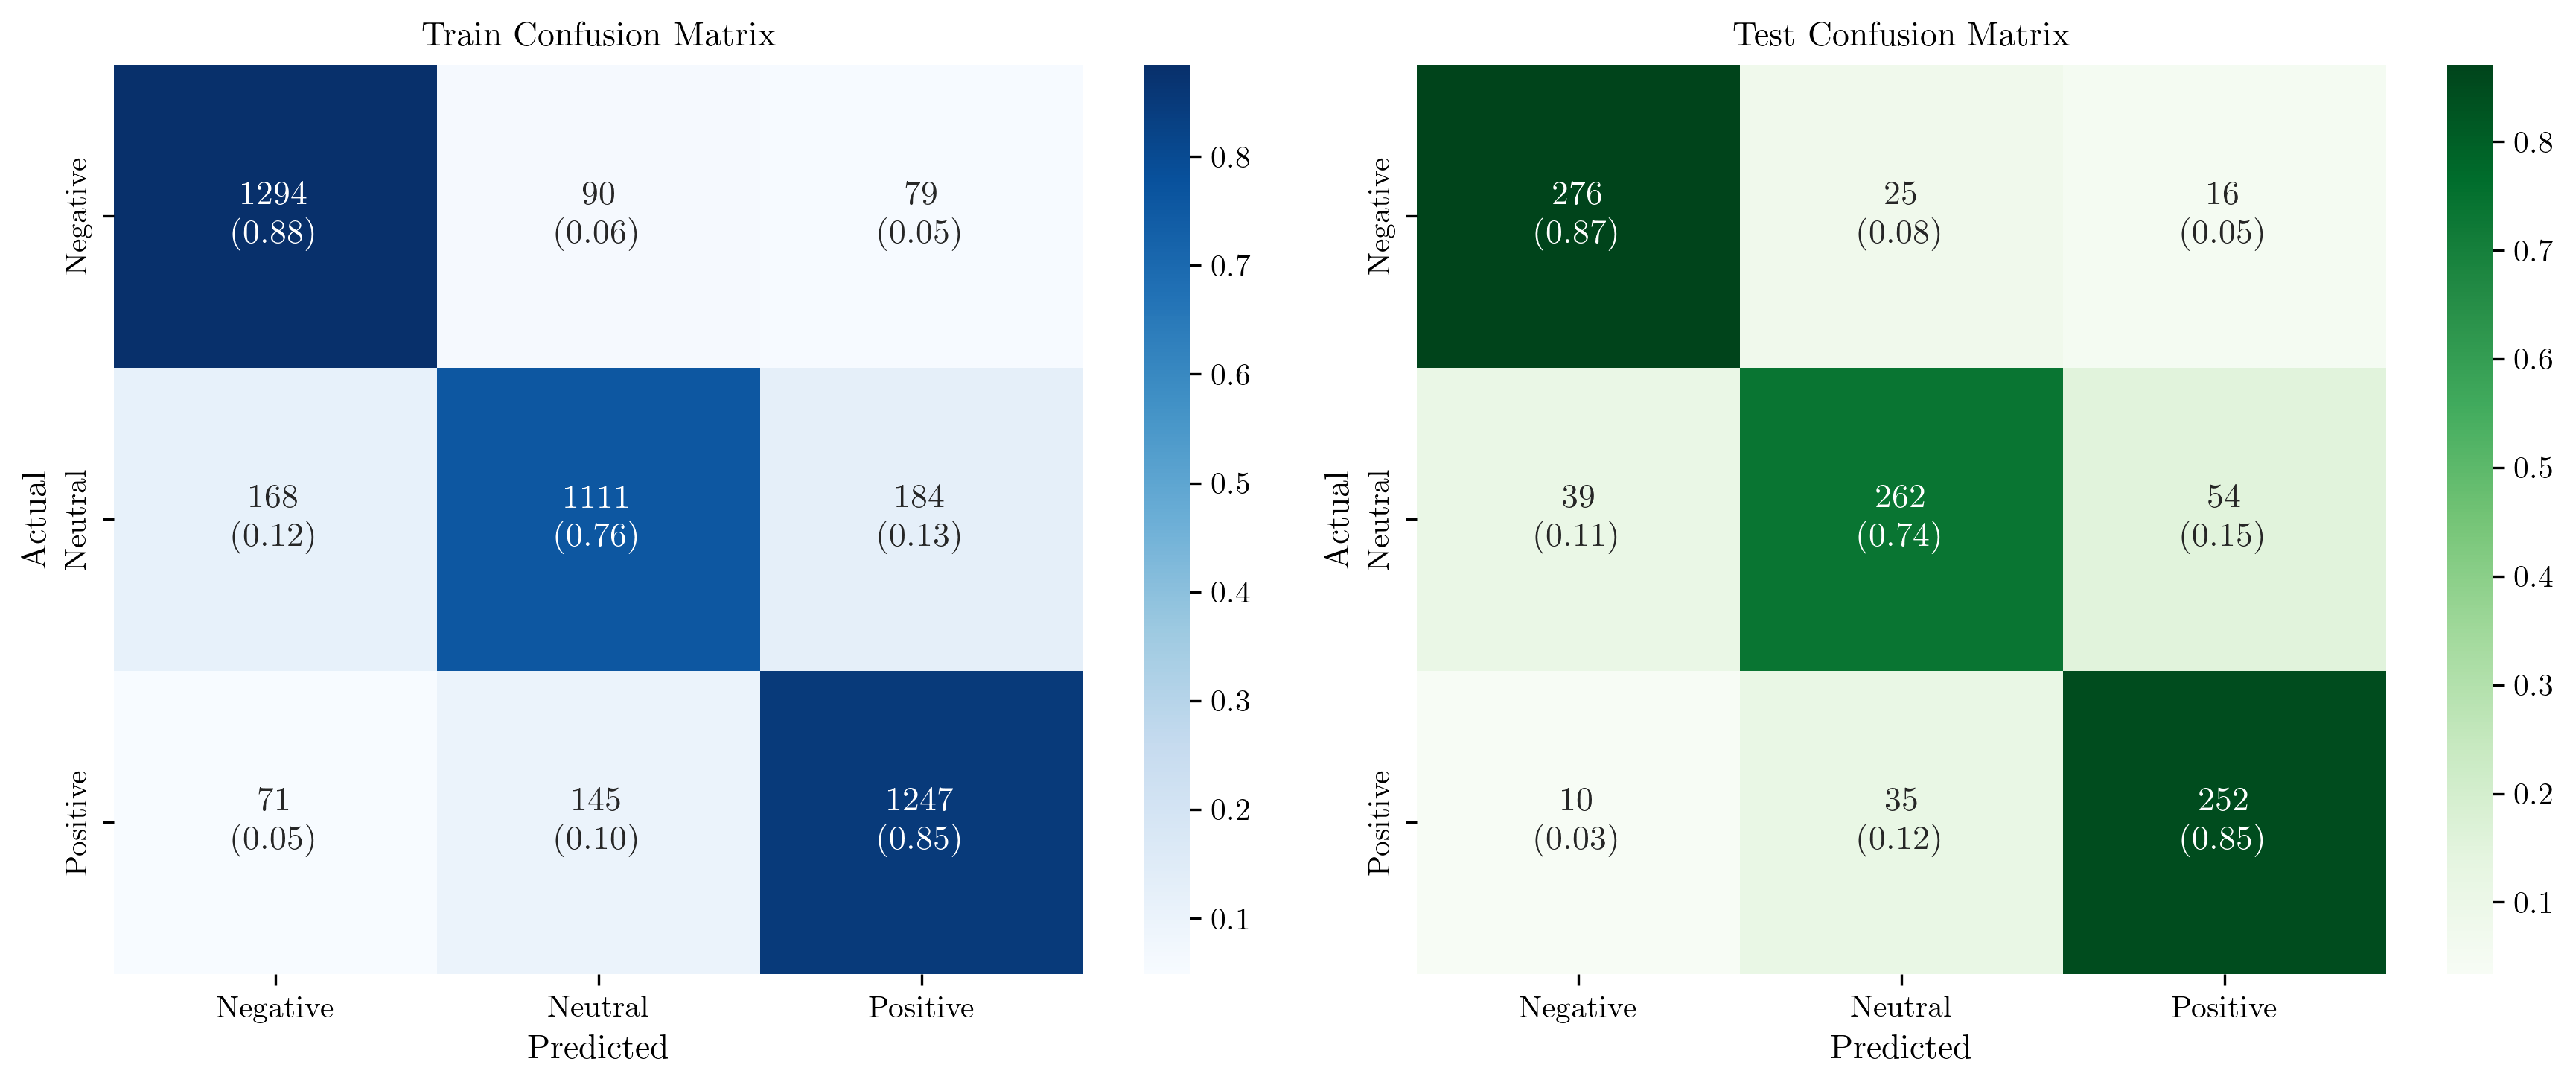
\includegraphics[width=1\textwidth]{figs/gdelt_confusion_matrix.png}
    \caption{Confusion matrices for sector-specific sentiment classification of GDELT quotes, with the training set shown on the left and the held-out test set on the right.}
    \label{fig:GDELT_confusion_matrix}
\end{figure}

\newpage

Table~\ref{tab:GDELT_macro_f1_sector} reports the macro-F1 score per sector on the held-out test set, showing that performance varies across sectors, ranging from a macro-F1 score of $0.88$ for Communication Services down to $0.72$ for Energy. Sectors with more standardized and domain-specific language, such as Consumer Staples and Utilities, tend to be easier to classify, whereas sectors like Energy, whose news frequently involves geopolitical context with ambiguous implications for sector performance, prove more challenging. These differences are a natural consequence of the underlying variability in news content and do not undermine the overall utility of the sentiment signal for the downstream portfolio analysis.

\begin{table}[ht]
\centering
\caption{Macro-F1 score per sector for GDELT sector-specific sentiment classification on the held-out test set.}
\label{tab:GDELT_macro_f1_sector}
\renewcommand{\arraystretch}{1.2}
\begin{tabular}{|l|c|c|}
\hline
\textbf{Sector} & \textbf{Macro-F1} & \textbf{Support} \\
\hline
Energy & 0.72 & 86 \\
Materials & 0.79 & 74 \\
Industrials & 0.84 & 90 \\
Consumer Discretionary & 0.80 & 92 \\
Consumer Staples & 0.86 & 102 \\
Health Care & 0.78 & 86 \\
Financials & 0.82 & 90 \\
Information Technology & 0.81 & 84 \\
Communication Services & 0.88 & 75 \\
Utilities & 0.85 & 91 \\
Real Estate & 0.79 & 99 \\
\hline
\end{tabular}
\end{table}
